%%%%%%%%%%%%%%%%%%%%%%%%%%%%%%%%%%%%%%%%%%%%%%%%%%%%%%%%%%%%%%%%%
\begin{slide}{Motivation: More Resolution where we really need it}
%%%%%%%%%%%%%%%%%%%%%%%%%%%%%%%%%%%%%%%%%%%%%%%%%%%%%%%%%%%%%%%%%

\vspace{0.5in}
\begin{center}
Precipitation rate on 2 November 2008\\
\includegraphics{plots/ppt.png}
\end{center}

\end{slide}

%%%%%%%%%%%%%%%%%%%%%%%%%%%%%%%%%%%%%%%%%%%%%%%%%%%%%%%%%%%%%%%%%
\begin{slide}{But fine scale detail is ubiquitous}
%%%%%%%%%%%%%%%%%%%%%%%%%%%%%%%%%%%%%%%%%%%%%%%%%%%%%%%%%%%%%%%%%

\begin{center}
NEODAAS GOES East 075.0W 2 Nov 2008 18:00hours Channel: 1 (Visible)
%Meteosat SEVIRI midday on 2 Nov 2008 Channel: 1 (0.56 - 0.71 $\mu m$ Visible) \\
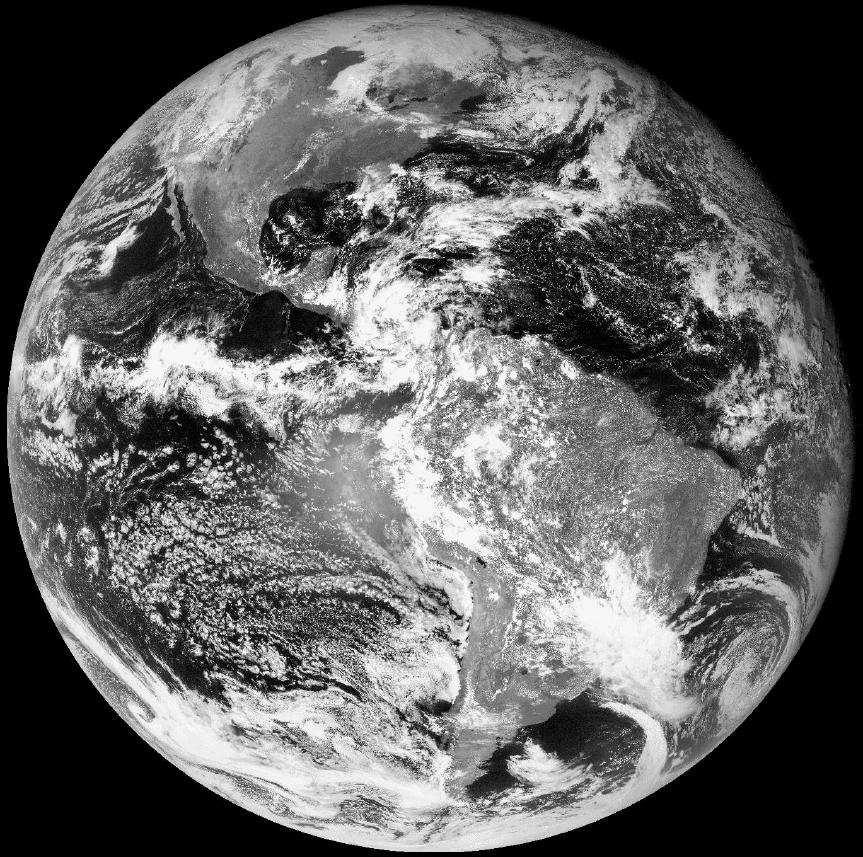
\includegraphics[scale=0.5]{plots/2008_11_2_1800_GOES12_1_S2.jpg}
\end{center}

\end{slide}

%%%%%%%%%%%%%%%%%%%%%%%%%%%%%%%%%%%%%%%%%%%%%%%%%%%%%%%%%%%%%%%%%%%%%%%
\begin{slide}{}
%%%%%%%%%%%%%%%%%%%%%%%%%%%%%%%%%%%%%%%%%%%%%%%%%%%%%%%%%%%%%%%%%%%%%%%

\begin{center}
\large
NICAM uses a hexagonal icosahedral mesh at fixed resolutions down to 3.5km on the Earth Simulator and captures features of tropical cloud clusters: \\
(see work of Masaki Satoh et al, JAMSTEC)

\vspace{20pt}
\begin{tabular}{cc}
NICAM at 3.5km & GMS/GOES-9 at Apr. 6, 2004, 00UTC\\
\includegraphics{plots/NICAM.png}
&
\includegraphics{plots/GOES-9.png}
\end{tabular}

\end{center}

\begin{list0}

    \item But these ``Grand Challenge'' experiments are too expensive for operations

    \item And 3.5km is still not really fine enough to {\it resolve} convection

\end{list0}

\end{slide}
